

\section{Vocabulaire et notations}

\subsection{Série numérique}

\begin{Def}\textbf{Série numérique}
    

Une série numérique est une somme abstraite infinie de scalaires (réels ou complexes), notée :
\[
\sum_{n > 0} u_n \quad \text{ou parfois} \quad \sum u_n.
\]

Parfois, les termes de cette somme ne sont pris en compte qu'à partir d'un certain indice $n_0$, auquel cas la série est notée :
\[
\sum_{n > n_0} u_n.
\]
\end{Def}

\begin{Def}\textbf{Somme partielle}\\

Pour tout entier $N$, la somme partielle de rang $N$ de la série $\sum u_n$ est le nombre :
\[
\sum_{n=0}^{N} u_n.
\]

Dans le cas plus général d'une série numérique de la forme $\sum_{n > n_0} u_n$, c'est pour tout entier $N > n_0$ que l'on définit la somme partielle de rang $N$ par la formule :
\[
\sum_{n = n_0}^{N} u_n.
\]
\end{Def}

\begin{Def}\textbf{Convergence}\\

Dire que la série $\sum_{n > n_0} u_n$ converge signifie que la suite des sommes partielles :
\[
\left( \sum_{n = n_0}^{N} u_n \right)_{N > n_0}
\]
converge.\\
La notion de divergence se transmet également.
\end{Def}

\begin{Rmq}
Soient $n_1$ et $n_2$ deux entiers avec $n_1 > n_2$.\\
On remarque que les suites de sommes partielles :
\[
\left( \sum_{n = n_1}^{N} u_n \right)_{N > n_1} \quad \text{et} \quad \left( \sum_{n = n_2}^{N} u_n \right)_{N > n_2}
\]
diffèrent d'une constante (à savoir $\sum_{n = n_2}^{n_1 - 1} u_n$).\\

Par conséquent, les séries $\sum_{n > n_1} u_n$ et $\sum_{n > n_2} u_n$ ont la même nature.\\
On dit aussi que les premiers termes de la série n'ont pas d'influence sur la nature de la série en question.\\



\end{Rmq}

\subsection{Somme d'une série convergente}

\begin{Def}\textbf{Somme d'une série numérique}

En cas de convergence, la limite de la suite des sommes partielles est appelée \textbf{la somme de la série}.
On note :
\[
\sum_{n=n_0}^{+\infty} u_n = \lim_{N \to +\infty} \sum_{n=n_0}^{N} u_n.
\]
\end{Def}

\begin{Prop}\textbf{Décalage}

Soit $\sum_{n > n_0} u_n$ une série convergente. Alors, pour tout entier $n_1 > n_0$, la série $\sum_{n > n_1} u_n$ converge aussi, et leurs sommes sont reliées par la formule :
\[
\sum_{n = n_0}^{+\infty} u_n = \sum_{n = n_0}^{n_1 - 1} u_n + \sum_{n = n_1}^{+\infty} u_n.
\]
\end{Prop}

\subsection{Reste d'une série convergente}

\begin{Def}\textbf{Reste d'une série convergente}

Soit $\sum_{n > n_0} u_n$ une série convergente.

Pour tout entier $N > n_0$, on appelle \textbf{reste d'ordre $N$} de cette série ce qui reste de la somme quand on lui a retiré la somme partielle de rang $N$ :
\[
\sum_{n = n_0}^{+\infty} u_n - \sum_{n = n_0}^{N} u_n = \sum_{n = N + 1}^{+\infty} u_n.
\]
La suite des restes d'une série convergente est une suite de limite nulle.
\end{Def}


\begin{Ex}

\begin{itemize}
  \item La \textbf{série nulle} $\sum_{n > 0} 0$ est convergente.
  
  Sa somme est nulle, de même que toutes ses sommes partielles et ses restes.
  
  \item Pour toute constante $\alpha \neq 0$, la série $\sum_{n > 0} \alpha$ est \textbf{divergente}.
  
  \item La série $\sum_{n > 0} (-1)^n$ est divergente.\newline
  En effet, pour tout $N \in \mathbb{N}$, la somme partielle de rang $N$ s'exprime ainsi :
  \[
  S_N = \sum_{n=0}^{N} (-1)^n = \frac{1 + (-1)^N}{2} = 
  \begin{cases}
    1 & \text{si } N \text{ est pair}, \\
    0 & \text{si } N \text{ est impair}.
  \end{cases}
  \]
  Les suites extraites $(S_{2k})_{k \in \mathbb{N}}$ et $(S_{2k+1})_{k \in \mathbb{N}}$ sont convergentes, de limites distinctes,\\ donc la suite $(S_N)_{N > 0}$ est divergente.

\end{itemize}
\end{Ex}


        
\newpage

\subsection{Opérations sur les séries}
\begin{Prop}\textbf{Somme de deux séries}\\
Soient $\sum u_n$ et $\sum v_n$ deux séries.\\

\begin{itemize}
\item La somme des séries est la série de terme général $u_n + v_n$.
\item Pour tout $\lambda \in \mathbb{R}$, alors $\lambda \sum u_n = \sum \lambda u_n$
\end{itemize}

Si $\sum u_n$ et $\sum v_n$ convergent, alors :
\[
\sum (u_n + v_n) \text{ converge et } \sum u_n + \sum v_n = \sum (u_n + v_n)
\]
\end{Prop}

\begin{Rmq}
- La somme d'une série convergente et d'une série divergente est divergente.
- Pour la somme de deux séries divergentes : pas de règle générale.\\

\end{Rmq}

\subsection{Divergence grossière}

\begin{Prop}\textbf{Divergence grossière}\\
Si la suite $(u_n)_{n > n_0}$ ne converge pas vers $0$, alors la série $\sum u_n$ est divergente.

On dit dans ce cas que cette série \textbf{diverge grossièrement}.
\end{Prop}
\bigskip

\begin{Rmq}
\textbf{Attention :} la réciproque est complètement fausse : il existe des séries divergentes dont le terme général tend vers 0, comme on le voit avec certaines séries de Riemann ou avec l'exemple du paragraphe précédent.
\end{Rmq}

        
\newpage

\subsection{QCM}

Pour chaque question, une seule réponse est correcte. 


\begin{enumerate}[label=\textbf{Q\arabic*.}, wide=0pt, itemsep=1.2em]

\item  
Une série numérique $\displaystyle \sum_{n=0}^{+\infty} u_n$ est :  
\begin{multicols}{2}
\begin{enumerate}[label=\alph*)]
  \item une suite de réels $u_n$ indexée par $n$.  
  \item la limite de la suite $u_n$ quand $n \to \infty$.  
  \item une somme infinie des termes $u_n$.  
  \item le produit infini $\displaystyle\prod_{n=0}^{+\infty} u_n$.  
\end{enumerate}
\end{multicols}
\item  
La somme partielle de rang $N$ de la série $\displaystyle \sum_{n=0}^{+\infty} u_n$ est :  
\begin{multicols}{2}
\begin{enumerate}[label=\alph*)]
  \item $\displaystyle S_N = \sum_{n=0}^{N} u_n$.  
  \item $\displaystyle S_N = \lim_{n\to N} u_n$.  
  \item $\displaystyle S_N = u_{N+1}+u_{N+2}+\cdots$.  
  \item $\displaystyle S_N = \int_0^N u_n\, dn$.  
\end{enumerate}
\end{multicols}
\item  
Le \textbf{reste} d'ordre $N$ de la série $\displaystyle \sum_{n=0}^{+\infty} u_n$ est défini par :  
\begin{multicols}{2}
\begin{enumerate}[label=\alph*)]
  \item $\displaystyle R_N = S_N - u_N$.  
  \item $\displaystyle R_N = \sum_{n=0}^{N} u_n$.  
  \item $\displaystyle R_N = \sum_{n=N+1}^{+\infty} u_n$.  
  \item $\displaystyle R_N = \lim_{M\to\infty} \sum_{n=N+1}^{M} u_n$.  
\end{enumerate}
\end{multicols}
\item  
Supposons que $\sum u_n$ converge. Que peut-on dire du reste $R_N$ quand $N \to \infty$ ?  
\begin{multicols}{2}
\begin{enumerate}[label=\alph*)]
  \item Il converge vers la somme totale de la série.  
  \item Il diverge vers $+\infty$.  
  \item Il converge vers 0.  
  \item Il oscille entre deux bornes.  
\end{enumerate}
\end{multicols}
\item  
Si la série $\sum u_n$ converge, alors :  
\begin{multicols}{2}
\begin{enumerate}[label=\alph*)]
  \item $u_n$ converge vers la somme de la série.  
  \item $u_n \to 0$ quand $n \to \infty$.  
  \item $\sum |u_n|$ converge aussi.  
  \item $u_n$ devient constant à partir d'un certain rang.  
\end{enumerate}
\end{multicols}
\item  
Deux séries $\sum_{n>n_0} u_n$ et $\sum_{n>n_1} u_n$ ayant des indices de départ différents : 
\begin{enumerate}[label=\alph*)]
  \item peuvent être de natures différentes (convergente/divergente).  
  \item sont toutes deux convergentes ou toutes deux divergentes.  
  \item convergentes si et seulement si $n_0 = n_1$.  
\end{enumerate}

\item  
On supprime un nombre fini de termes au début d'une série. Cela modifie :  
\begin{enumerate}[label=\alph*)]
  \item sa nature (convergence ou divergence).  
  \item sa somme, mais pas sa nature.  
  \item ni sa nature ni sa somme.  
  \item son reste de manière significative.  
\end{enumerate}

\end{enumerate}

\section{ Séries à connaître et à reconnaître}

\subsection{Série alternée}


\begin{Def}\textbf{Série alternée}\\
Les séries de la forme $\sum (-1)^n a_n$, avec $a_n \geq 0$, sont appelées alternées.
\end{Def}

\begin{Thm}[Leibniz]
\textbf{Critère spécial des séries alternées}\\
Soit $(u_n)_{n \in \mathbb{N}}$ une suite réelle décroissante qui converge vers 0.

Alors la série $\sum (-1)^n u_n$ est convergente.\\

De plus, pour tout entier $N$, le reste
\[
\sum_{n = N}^{+\infty} (-1)^n u_n
\]
a le même signe que $(-1)^N u_N$.

Enfin, pour tout entier $N$, on a la majoration :
\[
\left| \sum_{n = N}^{+\infty} (-1)^n u_n \right| \leq u_N. 
\]
\end{Thm}

\begin{Rmq}

\begin{enumerate}
  \item Si la suite $(u_n)_{n \in \mathbb{N}}$ converge vers 0 en croissant, alors les inégalités sur les sommes partielles sont renversées, mais les autres propriétés subsistent. En particulier, le signe du reste est toujours déterminé par le premier terme de la somme qui définit ce reste.\\
  
  \item Si la suite $(u_n)_{n \in \mathbb{N}}$ converge vers $0$ mais n'est décroissante qu'à partir d'un rang $n_0$, alors la série $\sum (-1)^n u_n$ converge aussi. La propriété sur le signe du reste n'est valable a priori que si $N \geq n_0$ ; il en va de même pour les inégalités sur les sommes partielles.\\
  
  \item Pour des séries absolument convergentes comme $\sum (-1)^n / n^2$ ou $\sum (-1)^n / n!$, la première partie de ce théorème est inutile ; cependant, les propriétés sur le signe du reste et l'encadrement de la somme peuvent être intéressantes.\\
\end{enumerate}
\end{Rmq}

% On a la réciproque du critère de base : une série alternée converge si et seulement si $\lim u_n = 0$.
\vspace{1em}
\hrule
\vspace{1em}
\exo[1]{Premier exemple} 
La série $\sum \frac{(-1)^n}{n}$ est-elle convergente ?\\


\vspace{1em}
\hrule
\vspace{1em}


\exo[2]{Estimation du reste}
Calculer une estimation du reste pour la somme partielle à l'ordre $N$ :
\[
\sum_{n=1}^{+\infty} \frac{(-1)^n}{n}.
\]
\vspace{1em}
\hrule
\vspace{1em}
\exo[2]{Converge ou diverge?}
Montrer que la série alternée
\[
\sum_{n=1}^{+\infty} (-1)^n \frac{\ln(n)}{n}
\]
converge ou diverge.\\
\vspace{1em}
\hrule
\vspace{1em}
\exo[2]{Converge ou diverge? bis}
Étudier la convergence de la série
\[
\sum_{n=1}^{+\infty} \frac{(-1)^n}{\sqrt{n}}.
\]
\vspace{1em}
\hrule
\vspace{1em}

  
\subsection{Série télescopique}

\begin{Prop}\textbf{Série télescopique}\\
Soit $(u_n)_{n > n_0}$ une suite numérique.

Soit un entier $n > n_0 + 1$. Un \textit{télescopage} donne :
\[
u_n = u_{n_0} + \sum_{k = n_0}^{n - 1} (u_{k+1} - u_k).
\]

Ainsi, la convergence de la suite $(u_n)_{n > n_0}$ équivaut à celle de la \textbf{série des différences}
\[
\sum_{k > n_0} (u_{k+1} - u_k).
\]
\end{Prop}

\begin{Ex} La suite $(\ln(n))_{n > 2}$ est divergente, donc sa série des différences est divergente.\\
Cette série s'écrit :
\[
\sum_{n > 2} \ln\left(1 + \frac{1}{n}\right).
\]
\end{Ex}
\begin{Ex}Prenons un nombre complexe $z$ tel que $|z| < 1$.\\ On sait que la suite $(z^n)_{n \in \mathbb{N}}$ converge (vers 0).\\ On en déduit que la série $\sum (z^n - z^{n+1})$ est convergente.

En simplifiant par la constante non nulle $1 - z$, on en déduit que la série $\sum z^n$ est convergente.\\
\end{Ex}
\vspace{1em}
\hrule
\vspace{1em}
\exo[1]{Série télescopique}
Étudier la convergence et calculer la somme de la série télescopique
\[
\sum_{n=1}^{+\infty} \left( \frac{1}{n} - \frac{1}{n+1} \right).
\]

\vspace{1em}
\hrule
\vspace{1em}

        
\newpage

\subsection{Série de référence : série géométrique, série de Riemann, et série exponentielle}


\textbf{Série géométrique}

\begin{Def}\textbf{Les séries géométriques}\\

Soit $z \in \mathbb{C}$. On étudie la série géométrique :
\[
\sum_{n=0}^{+\infty} z^n.
\]
\end{Def}

\begin{Prop}\textbf{Convergence d'une série géométrique}\\
\begin{itemize}
    \item  Si $|z| \geq 1$, alors la série $\sum z^n$ diverge grossièrement (le terme général ne tend pas vers 0).
    \item  Si $|z| < 1$, alors la série converge et sa somme vaut :
    \[
    \sum_{n=0}^{+\infty} z^n = \frac{1}{1 - z}.
    \]
\end{itemize}

Plus généralement, dès que la raison $r$ a un module strictement inférieur à 1, on a :
\[
\text{somme} = (\text{premier terme}) \times \frac{1}{1 - r}.
\]
\end{Prop}

\begin{Ex}
$\sum_{n=2}^{+\infty} \frac{3}{2^{2n+1}} = \frac{3}{32} \times \frac{1}{1 - \frac{1}{4}} = \frac{1}{8}.$\\
\end{Ex}
\vspace{1em}
\hrule
\vspace{1em}
\exo{Application}
 Calculer la somme de la série géométrique
\[
\sum_{n=0}^{+\infty} \left(\frac{1}{3}\right)^n.
\]
\vspace{1em}
\hrule
\vspace{1em}

\newpage

\textbf{Série de Riemann}
\begin{Def}\textbf{Les séries de Riemann}

Soit $\alpha \in \mathbb{R}$. On appelle série de Riemann de paramètre $\alpha$ la série :
\[
\sum_{n=1}^{+\infty} \frac{1}{n^\alpha}.
\]

\end{Def}

\begin{Prop}\textbf{Convergence des séries de Riemann}

\begin{itemize}
    \item  Si $\alpha \leq 1$, la série diverge.
    \item Si $\alpha > 1$, la série converge.
\end{itemize}
\end{Prop}

\vspace{1em}
\hrule
\vspace{1em}
\exo[1]{Pont aux ânes}
Donner la nature des séries suivantes:
\begin{multicols}{2}
\begin{enumerate}[label=\alph*)]
    \item 

\[
\sum_{n=1}^{+\infty} \frac{1}{n^{3/4}},
\]
\item
\[
\sum_{n=1}^{+\infty} \frac{1}{n^{3/2}}\]
\item
\[
\sum_{n=1}^{+\infty} \frac{1}{n^2},\]
\item
\[
\sum_{n=1}^{+\infty} \frac{1}{n},\]
\item
\[
\sum_{n=1}^{+\infty} \frac{1}{\sqrt{n}}, 
\]
\item
\[
\sum_{n=1}^{+\infty} \frac{1}{n^3},
\]
\end{enumerate}
    
\end{multicols}
\vspace{1em}
\hrule
\vspace{1em}

\exo[2]{Convergence ou absolue convergence}

Montrer que la série
\[
\sum_{n=1}^{+\infty} \frac{(-1)^n}{n^2}
\]
est absolument convergente et calculer une majoration du reste après $N$ termes.

\vspace{1em}
\hrule
\vspace{1em}

\exo[1]{Série de Riemann}
 Étudier la convergence de la série de Riemann
\[
\sum_{n=1}^{+\infty} \frac{1}{n^\alpha}
\]
en fonction du paramètre réel $\alpha > 0$.
\vspace{1em}
\hrule
\vspace{1em}
\exo[2]{Convergence d'une série de Riemann}
Déterminer la nature (convergence/divergence) de la série suivante pour $\beta > 0$.
\[
\sum_{n=2}^{+\infty} \frac{1}{n \ln(n)^\beta}
\]

\vspace{1em}
\hrule
\vspace{1em}
\textbf{Série exponentielle}

\begin{Def}\textbf{La série exponentielle}\\
Pour tout $z \in \mathbb{C}$, la série exponentielle converge et on a :
\[
\sum_{n=0}^{+\infty} \frac{z^n}{n!} = e^z.
\]
\end{Def}

\begin{Rmq}Il ne faut pas oublier que la somme commence à l'indice $n=0$. Si on commence à $n=1$, la formule est fausse pour $z=0$.
\end{Rmq}

\textbf{Démonstration (par Taylor avec reste intégral)}

Soit $z \in \mathbb{C}$, et définissons $f(t) = e^{tz}$. Cette fonction est de classe $\mathcal{C}^\infty$ sur $\mathbb{R}$.

Appliquons la formule de Taylor avec reste intégral entre 0 et $x$ à l'ordre $n$ :
\[
f(x) = \sum_{k=0}^n \frac{f^{(k)}(0)}{k!} x^k + \int_0^x \frac{f^{(n+1)}(t)}{n!} (x - t)^n \, dt.
\]

Comme $f^{(k)}(t) = z^k e^{tz}$, on obtient pour $x=1$ :
\[
e^z = \sum_{k=0}^n \frac{z^k}{k!} + \frac{z^{n+1}}{n!} \int_0^1 e^{tz} (1 - t)^n dt.
\]

Par inégalité triangulaire :
\[
\left| e^z - \sum_{k=0}^n \frac{z^k}{k!} \right| \leq \frac{|z|^{n+1}}{n!} \int_0^1 |e^{tz}| (1 - t)^n dt.
\]

Or, $|e^{tz}| = e^{t \Re(z)} \leq e^{|\Re(z)|}$ pour $t \in [0,1]$.

Ainsi :
\[
\left| e^z - \sum_{k=0}^n \frac{z^k}{k!} \right| \leq \frac{|z|^{n+1} e^{|\Re(z)|}}{(n+1)!}.
\]

Ce majorant tend vers 0 quand $n \to +\infty$, ce qui prouve la convergence de la série exponentielle.\\



\vspace{1em}
\hrule
\vspace{1em}


\exo[2]{Série exponentielle}
Montrer que la série exponentielle
\[
\sum_{n=0}^{+\infty} \frac{z^n}{n!}
\]
converge pour tout $z \in \mathbb{C}$ et que sa somme est égale à $e^z$.\\

\vspace{1em}
\hrule
\vspace{1em}


\subsection{QCM}

Pour chaque question, une seule réponse est correcte. \\

\begin{enumerate}[label=\textbf{Q\arabic*.}, wide=0pt, itemsep=1.5em]

\item Une série numérique $\sum_{n=0}^{+\infty} u_n$ converge si :

\begin{enumerate}[label=\alph*)]
  \item $u_n \underset{n \to \infty}{\longrightarrow} 0$  
  \item La suite des sommes partielles $\displaystyle S_n = \sum_{k=0}^{n} u_k$ admet une limite finie  
  \item Tous les termes $u_n$ sont positifs  
  \item $u_n$ est décroissante  
\end{enumerate}

\item La somme partielle d'ordre $n$ d'une série $\sum u_k$ est :
\begin{multicols}{2}
\begin{enumerate}[label=\alph*)]
  \item $\displaystyle S_n = u_n$  
  \item $\displaystyle S_n = \sum_{k=0}^{n} u_k$  
  \item $\displaystyle S_n = \lim_{k \to n} u_k$  
  \item $\displaystyle S_n = \sum_{k=n}^{+\infty} u_k$  
\end{enumerate}
\end{multicols}
\item Le reste d'ordre $n$ d'une série convergente $\sum u_k$ est :
\begin{multicols}{2}
\begin{enumerate}[label=\alph*)]
  \item $\displaystyle R_n = \sum_{k=n}^{+\infty} u_k$  
  \item $\displaystyle R_n = \sum_{k=0}^{n} u_k$  
  \item $\displaystyle R_n = u_n$  
  \item $\displaystyle R_n = S_n - S_{n-1}$  
\end{enumerate}
\end{multicols}
\item La série géométrique $\sum_{n=0}^{+\infty} z^n$ converge si :
\begin{multicols}{2}
\begin{enumerate}[label=\alph*)]
  \item $|z| < 1$  
  \item $|z| = 1$  
  \item $|z| > 1$  
  \item $z$ est réel négatif  
\end{enumerate}
\end{multicols}
\item Pour $|z| < 1$, on a : $\sum_{n=0}^{+\infty} z^n =$
\begin{multicols}{2}
\begin{enumerate}[label=\alph*)]
  \item $\dfrac{1}{1 - z}$  
  \item $-\ln(1 - z)$  
  \item $e^z$  
  \item $1 - z + z^2 - z^3 + \cdots$  
\end{enumerate}
\end{multicols}
\item La série de Riemann $\sum_{n=1}^{+\infty} \dfrac{1}{n^\alpha}$ converge si :
\begin{multicols}{2}
\begin{enumerate}[label=\alph*)]
  \item $\alpha = 1$  
  \item $\alpha < 1$  
  \item $\alpha > 1$  
  \item $\alpha \leq 0$  
\end{enumerate}
\end{multicols}
\item La série alternée $\sum_{n=0}^{+\infty} (-1)^n u_n$ converge si :
\begin{multicols}{2}
\begin{enumerate}[label=\alph*)]
  \item $u_n$ est croissante et tend vers 0  
  \item $u_n$ décroît vers 0  
  \item $u_n$ est constant  
  \item $u_n \underset{n \to \infty}{\longrightarrow} 0$ sans condition  
\end{enumerate}
\end{multicols}

\item Si $\sum_{n=0}^{+\infty} (-1)^n u_n$ est une série alternée vérifiant les conditions du théorème de Leibniz, alors pour tout $N$ :
\begin{multicols}{2}
\begin{enumerate}[label=\alph*)]
  \item Le reste $R_N$ est nul  
  \item Le signe du reste est celui de $(-1)^N u_N$  
  \item $|R_N| \leq u_0$  
  \item $R_N > u_N$.\\  
\end{enumerate}
\end{multicols}
  \item La série $\displaystyle \sum_{n=1}^{+\infty} \frac{(-1)^n}{n}$ :
\begin{enumerate}[label=\alph*)]
    \item Diverge car son terme général ne tend pas vers 0  
    \item Converge absolument  
    \item Converge mais pas absolument  
    \item Est télescopique  
  \end{enumerate}

  \item Soit $\displaystyle \sum_{n=1}^{+\infty} (-1)^n u_n$, avec $u_n > 0$, décroissante et tendant vers 0. Alors :
\begin{enumerate}[label=\alph*)]
    \item La série diverge  
    \item Le reste $R_N$ vérifie $|R_N| \leq u_N$  
    \item Le reste est nul  
    \item La série est absolument convergente  
  \end{enumerate}

  \item La série $\displaystyle \sum_{n=1}^{+\infty} \frac{(-1)^{n+1}}{n^2}$ :
  \begin{enumerate}[label=\alph*)]
    \item Diverge  
    \item Converge conditionnellement  
    \item Converge absolument  
    \item Est télescopique  
  \end{enumerate}



  \item La série $\displaystyle \sum_{n=1}^{+\infty} \left( \frac{1}{n} - \frac{1}{n+1} \right)$ :
\begin{enumerate}[label=\alph*)]
    \item Converge et sa somme vaut 1  
    \item Diverge  
    \item Est alternée  
    \item Converge et sa somme vaut $\ln 2$  
  \end{enumerate}

  \item On pose $u_n = \frac{1}{n(n+1)}$. Alors la série $\sum u_n$ :
\begin{enumerate}[label=\alph*)]
    \item Est une série alternée  
    \item Est télescopique et converge vers 1  
    \item Diverge  
    \item Converge mais sans expression explicite  
  \end{enumerate}

  \newpage

  \item La série $\displaystyle \sum_{n=1}^{+\infty} \left( \ln(n+1) - \ln(n) \right)$ :
\begin{enumerate}[label=\alph*)]
    \item Est alternée  
    \item Converge vers $\ln 2$  
    \item Est télescopique et diverge  
    \item Est absolument convergente 
  \end{enumerate}
\end{enumerate}




\section{Séries à terme positif}

\subsection{Comparaison série-intégrale (méthode des rectangles)}

\begin{Prop}\textbf{Comparaison série-intégrale}\\

Soient $n_0 \in \mathbb{N}$ et $f : [n_0, +\infty[ \to \mathbb{R}_+$ une fonction continue, décroissante et positive.

Alors la série 
\[
\sum_{n = n_0}^{+\infty} f(n)
\]
converge si et seulement si la suite 
\[
\left( \int_{n_0}^{n} f(x)\, dx \right)_{n \geq n_0}
\]
converge.\\
\end{Prop}


Soit une fonction $f$ définie sur un intervalle de la forme $[a, +\infty[$ et à valeurs dans les réels positifs. On  suppose $f$ décroissante\footnote{Ou croissante. Cela ne fait que renverser le sens des inégalités.}.

\begin{center}
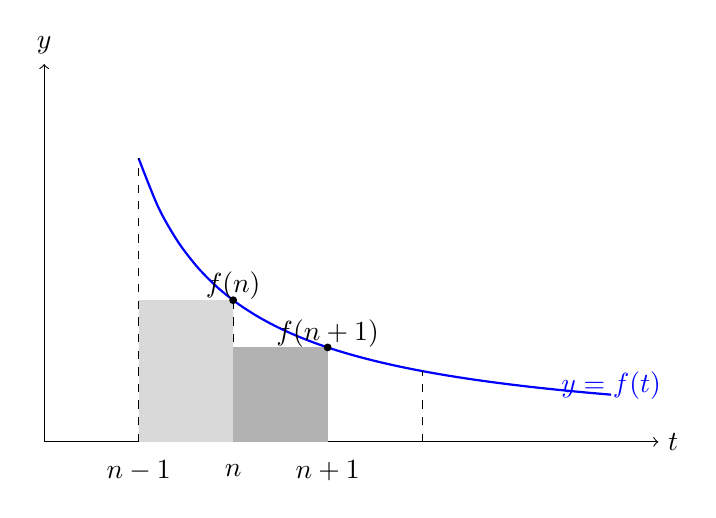
\begin{tikzpicture}[scale=1.2]
  % Axes
  \draw[->] (0,0) -- (6.5,0) node[right] {$t$};
  \draw[->] (0,0) -- (0,4) node[above] {$y$};

  % Courbe décroissante
  \draw[thick, domain=1:6, smooth, variable=\x, blue] plot ({\x}, {3/(\x)});

  % Lignes verticales
  \draw[dashed] (1,0) -- (1,3);
  \draw[dashed] (2,0) -- (2,1.5);
  \draw[dashed] (3,0) -- (3,1);
  \draw[dashed] (4,0) -- (4,0.75);

  % Rectangles
  \fill[gray!30] (1,0) rectangle (2,1.5); % f(2) rectangle
  \fill[gray!60] (2,0) rectangle (3,1);   % f(3) rectangle

  % Points f(n) and f(n-1)
  \node at (2,1.5)[circle,fill,inner sep=1pt]{};
  \node at (3,1)[circle,fill,inner sep=1pt]{};
  \node at (2,1.65) {$f(n)$};
  \node at (3,1.15) {$f(n+1)$};

  % Labels
  \node at (1,-0.3) {$n-1$};
  \node at (2,-0.3) {$n$};
  \node at (3,-0.3) {$n+1$};
  \node[blue] at (6,0.6) {$y = f(t)$};
\end{tikzpicture}

\vspace{0.3cm}
\textit{Méthode des rectangles pour $f$ décroissante}
\end{center}

\newpage

\textbf{Inégalités fondamentales}

Si $f$ est décroissante et $n > a+1$, alors :
\[
f(n) \leq \int_{n-1}^{n} f(t) \, dt
\qquad \text{et} \qquad
f(n) \geq \int_{n}^{n+1} f(t) \, dt.
\]

\paragraph{Justification formelle.}

Soit $n > a + 1$. La décroissance de $f$ implique que :
\[
\forall t \in [n-1,n], \quad f(n) \leq f(t).
\]
Donc, par croissance de l'intégrale :
\[
\int_{n-1}^{n} f(n) \, dt \leq \int_{n-1}^{n} f(t) \, dt.
\]
Or, l'intégrale de la fonction constante $f(n)$ sur $[n-1,n]$ vaut $f(n) \times 1 = f(n)$, donc :
\[
f(n) \leq \int_{n-1}^{n} f(t) \, dt.
\]

De même, l'encadrement supérieur s'obtient via :
\[
f(n) \geq \int_{n}^{n+1} f(t) \, dt.
\]

\subsubsection*{Application aux fonctions puissances}

Prenons $f_\alpha(t) = \dfrac{1}{t^\alpha}$ avec $\alpha > 0$, sur $[1, +\infty[$. On a alors :
\[
\int_1^n f_\alpha(t)\, dt
= \sum_{k=1}^{n-1} \int_k^{k+1} f_\alpha(t)\, dt
\leq \sum_{k=1}^{n-1} f_\alpha(k),
\]
et aussi :
\[
\int_1^n f_\alpha(t)\, dt
= \sum_{k=2}^{n} \int_{k-1}^{k} f_\alpha(t)\, dt
\geq \sum_{k=2}^{n} f_\alpha(k).
\]

D'où l'encadrement :
\[
f_\alpha(n) + \int_1^n f_\alpha(t)\, dt
\leq \sum_{k=1}^{n} f_\alpha(k)
\leq f_\alpha(1) + \int_1^n f_\alpha(t)\, dt.
\]

\textit{Cet encadrement donne une approximation précise de la somme partielle par l'intégrale, très utile dans l'étude des séries de Riemann.}



\newpage

\subsection{Critère de Cauchy}

\begin{Prop}\textbf{Critère de Cauchy}\\

Soit la série $(\sum u_n)$ une série à termes positifs ou nuls. Soit $l$ tel que
\[
\underset{n\to +\infty}{\lim}( \sqrt[n]{u_n}) =l
\]
\begin{itemize}
\item Si $l < 1$, la série converge.
\item Si $l > 1$, la série diverge.
\item Si $l = 1$, pas de conclusion.\\
\end{itemize}

\end{Prop}
\vspace{1em}
\hrule
\vspace{1em}

\exo[2]{Application}
La série $\sum \frac{x^n}{n^n}$ est-elle convergente ?
\vspace{1em}
\hrule
\vspace{1em}

\subsection{Théorèmes de comparaison pour les séries à termes positifs}

\begin{Prop}\textbf{Proposition fondamentale}\\

Si la suite $(u_n)_{n > n_0}$ est à termes réels positifs, alors la suite des sommes partielles est croissante à partir du rang $n_0$, donc elle admet une limite.\\

Si la suite des sommes partielles est majorée, on peut en déduire qu'elle converge ; la série $\sum u_n$ converge.\\

Dans le cas contraire, cette série diverge et la suite des sommes partielles tend vers $+\infty$.\\
\end{Prop}





\begin{Prop}\textbf{Critères de comparaison}\\
On considère deux suites réelles $(u_n)_{n > n_0}$ et $(v_n)_{n > n_1}$.

On suppose qu'il existe un indice entier $n_2 > \max(n_0, n_1)$ vérifiant l'encadrement :
\[
\forall n > n_2,\quad 0 \leq u_n \leq v_n.
\]

Si la série $\sum v_n$ converge, alors la série $\sum u_n$ converge aussi. Dans ce cas, on peut également écrire :
\[
\sum_{n = n_2}^{+\infty} u_n \leq \sum_{n = n_2}^{+\infty} v_n.
\]

Par contraposition, si la série $\sum u_n$ diverge, alors la série $\sum v_n$ diverge aussi.
\end{Prop}

\medskip

\textbf{Démonstration.} On suppose que la série $\sum v_n$ converge. Pour tout entier $N > n_2$, on a :
\[
\sum_{n = n_2}^{N} u_n \leq \sum_{n = n_2}^{N} v_n \leq \sum_{n = n_2}^{+\infty} v_n.
\]
La suite des sommes partielles de la série $\sum_{n > n_2} u_n$ est donc majorée. Comme elle est aussi croissante, elle converge. La série $\sum u_n$ est donc convergente. \hfill $\heartsuit$

\begin{Prop}\textbf{Critère de négligeabilité}\\

On reprend les notations précédentes. On suppose que les deux suites ont leurs termes positifs à partir d'un certain rang. On fait de plus l'hypothèse suivante :
\[
u_n = o_{n \to +\infty}(v_n).
\]

Si la série $\sum v_n$ converge, alors la série $\sum u_n$ converge aussi.

Par contraposition, si la série $\sum u_n$ diverge, alors la série $\sum v_n$ diverge aussi.

\end{Prop}

\textbf{Démonstration.} L'hypothèse de négligeabilité implique qu'il existe un rang $n_3$ tel que pour tout $n > n_3$, on ait :
\[
u_n \leq v_n.
\]
On peut alors appliquer le critère de domination. \hfill $\heartsuit$



\begin{Prop}\textbf{Critère des équivalents}\\
On suppose que les deux suites ont leurs termes positifs à partir d'un certain rang, et que $u_n \sim v_n$ quand $n \to +\infty$.

Alors les séries $\sum u_n$ et $\sum v_n$ ont la même nature.

\end{Prop}

\textbf{Démonstration.} Le fait que $u_n \sim v_n$ signifie qu'il existe un rang $n_3$ tel que pour tout $n > n_3$, on ait :
\[
u_n \leq 2v_n \quad \text{et} \quad v_n \leq 2u_n.
\]

Le critère de domination permet d'en déduire que si l'une des deux séries $\sum u_n$ ou $\sum v_n$ converge, alors l'autre aussi.

Les deux séries ont donc la même nature. \hfill $\heartsuit$




\section{Convergence absolue}

\begin{Def}\textbf{Convergence absolue}\\

Étant donnée une suite complexe $(z_n)_{n > n_0}$, dire que la série $\sum z_n$ \textbf{converge absolument} signifie que la série $\sum |z_n|$ converge.\\

\end{Def}

\begin{Thm}

La convergence absolue implique la convergence.
\end{Thm}

\begin{Rmq}
Autrement dit, la convergence de la série $\sum |z_n|$ implique celle de la série $\sum z_n$.

De plus, dans ce cas, on a l'inégalité triangulaire infinie :
\[
\left| \sum_{n = n_0}^{+\infty} z_n \right| \leq \sum_{n = n_0}^{+\infty} |z_n|.
\]
\end{Rmq}

\begin{Ex}
Les séries suivantes convergent car elles convergent absolument :
\[
\sum_{n > 1} \frac{(-1)^n}{n^2}, \quad \sum_{n > 1} \frac{e^{i \ln(n)}}{2^n}.
\]
\end{Ex}

\begin{Rmq}
\textbf{Attention.} Il n'y a pas de notion de divergence absolue. Si la série $\sum |z_n|$ est divergente, on ne peut rien en conclure quant à la nature de la série $\sum z_n$.
\end{Rmq}

\textbf{Démonstration du théorème}\\

\paragraph{Premier cas : suites à valeurs réelles.} Soit $(u_n)_{n \in \mathbb{N}}$ une suite réelle, et on suppose que la série $\sum |u_n|$ converge.

On remarque alors l'encadrement :
\[
\forall n \in \mathbb{N},\quad 0 \leq |u_n| - u_n \leq 2|u_n|.
\]
Par comparaison à termes positifs, la série $\sum (|u_n| - u_n)$ est convergente.

L'identité $u_n = |u_n| - (|u_n| - u_n)$ permet d'en déduire que la série $\sum u_n$ est convergente.

\paragraph{Cas général : suites à valeurs complexes.} Soit $(z_n)_{n \in \mathbb{N}}$ une suite complexe. On suppose que la série $\sum |z_n|$ converge.

Pour tout $n \in \mathbb{N}$, on connaît les majorations :
\[
| \Re(z_n) | \leq |z_n|, \quad | \Im(z_n) | \leq |z_n|.
\]

On en déduit que les séries $\sum | \Re(z_n) |$ et $\sum | \Im(z_n) |$ convergent.

En utilisant le cas réel, on en déduit que les séries $\sum \Re(z_n)$ et $\sum \Im(z_n)$ convergent.

Enfin, la relation $z_n = \Re(z_n) + i \Im(z_n)$ permet de conclure que la série $\sum z_n$ est convergente. \hfill $\heartsuit$

\subsection{Critère de d'Alembert}
\begin{Prop}\textbf{Critère de d'Alembert}\\
    

Soit $\sum u_n$ une série à termes strictement positifs. On examine :
\[
\ell = \lim \frac{u_{n+1}}{u_n}
\]
- Si $\ell < 1$ alors la série converge.

- Si $\ell > 1$ elle diverge.

- Si $\ell = 1$ : indéterminé.
\end{Prop}

\vspace{1em}
\hrule
\vspace{1em}
\exo[2]{Première application}
La série $(\sum \frac{n^2}{x^n})$ est-elle convergente ?\\


\vspace{1em}
\hrule
\vspace{1em}

\newpage

\subsection{Suite du critère de d'Alembert}

En exploitant le fait que les $u_k$ sont strictement positifs et en itérant cette inégalité, on obtient :
\[
\forall n > n_0,\quad u_n \leq r^{n - n_0} u_{n_0}.
\]

Les inégalités $0 \leq r < 1$ donnent la convergence de la série $\sum r^n$. Par comparaison de séries à termes positifs, on en déduit que la série $\sum u_n$ est convergente.

\paragraph{Deuxième cas.} On se place dans le cadre de l'hypothèse $\ell > 1$. La définition de la limite donne cette fois l'existence d'un indice $n_0$ tel que :
\[
\forall n > n_0,\quad \frac{u_{n+1}}{u_n} > 1.
\]
On en déduit alors la minoration :
\[
\forall n > n_0,\quad u_n \geq u_{n_0},
\]
et cette minoration empêche la suite $(u_n)_{n \in \mathbb{N}}$ de tendre vers 0. La série $\sum u_n$ est donc grossièrement divergente.

\paragraph{Troisième cas.} Toutes les séries de Riemann donnent la valeur $\ell = 1$. Certaines d'entre elles convergent, d'autres divergent. Voilà pourquoi le cas $\ell = 1$ n'est pas conclusif. \hfill $\heartsuit$


\subsection{Adaptation des critères de comparaison}

\subsubsection{Critère de domination }

Soit $(z_n)_{n > n_0}$ une suite complexe. Soit $(u_n)_{n > n_1}$ une suite réelle positive.

On suppose que $z_n = O(u_n)$ et que la série $\sum u_n$ converge.

Alors la série $\sum z_n$ converge absolument, donc elle converge.

\subsubsection{Critère de négligeabilité }

Soit $(z_n)_{n > n_0}$ une suite complexe. Soit $(u_n)_{n > n_1}$ une suite réelle positive.

On suppose que $z_n = o(u_n)$ et que la série $\sum u_n$ converge.

Alors la série $\sum z_n$ converge absolument, donc elle converge.

\subsubsection{Critère des équivalents }

Soit $(z_n)_{n > n_0}$ une suite complexe. Soit $(u_n)_{n > n_1}$ une suite réelle positive.

On suppose que $|z_n| \sim u_n$ et que la série $\sum u_n$ converge.

Alors la série $\sum z_n$ converge absolument, donc elle converge.

\subsubsection{Règle de d'Alembert (adaptée)}

Soit $(z_n)_{n > n_0}$ une suite complexe, dont les termes sont tous non nuls à partir d'un certain rang. On suppose que le quotient
\[
\left| \frac{z_{n+1}}{z_n} \right|
\]
admet une limite $\ell$ quand $n \to +\infty$.

\begin{itemize}
  \item Si $\ell < 1$, alors la série $\sum |z_n|$ converge, donc la série $\sum z_n$ converge.
  \item Si $\ell > 1$, alors la suite $(|z_n|)_{n > n_0}$ ne tend pas vers 0, donc la série $\sum z_n$ diverge grossièrement.
  \item Si $\ell = 1$, aucune conclusion n'est possible. \hfill $\heartsuit$
\end{itemize}

\subsection{QCM}

Pour chaque question, une seule réponse est correcte.\\

\begin{enumerate}[label=\textbf{Q\arabic*.}]

\item La méthode des rectangles pour une fonction décroissante positive $f$ sur $[a,+\infty[$ permet de comparer la série $\sum_{n=a}^{+\infty} f(n)$ avec :
\begin{multicols}{2}
\begin{enumerate}[label=\alph*)]
    \item L'intégrale $\displaystyle \int_a^{+\infty} f(t) \, dt$  
    \item La série $\displaystyle \sum_{n=a}^{+\infty} \int_n^{n+1} f(t) \, dt$  
    \item La somme partielle $\sum_{k=a}^n f(k)$ uniquement  
    \item L'intégrale $\displaystyle \int_0^a f(t) \, dt$
\end{enumerate}
\end{multicols}

\item Selon la méthode des rectangles, si $f$ est décroissante positive, alors pour tout entier $n > a$ on a l'encadrement :
\[
f(n) \leq \int_{n-1}^n f(t) \, dt \quad \text{et} \quad \int_n^{n+1} f(t) \, dt \leq f(n)
\]
Cette propriété permet de conclure que :
\begin{enumerate}[label=\alph*)]
    \item La convergence de la série $\sum f(n)$ équivaut à celle de l'intégrale impropre $\int_a^{+\infty} f(t) dt$  
    \item La série $\sum f(n)$ diverge toujours  
    \item La série $\sum f(n)$ converge uniquement si $f$ est bornée  
    \item La série $\sum f(n)$ converge si et seulement si $\lim_{n \to \infty} f(n) = 0$
\end{enumerate}

\item Le critère de d'Alembert appliqué à une série $\sum u_n$ à termes positifs repose sur l'étude de la limite de :
\begin{multicols}{2}
\begin{enumerate}[label=\alph*)]
    \item $\displaystyle \lim_{n \to \infty} \frac{u_n}{u_{n+1}}$  
    \item $\displaystyle \lim_{n \to \infty} \frac{u_{n+1}}{u_n}$  
    \item $\displaystyle \lim_{n \to \infty} u_n$  
    \item $\displaystyle \lim_{n \to \infty} \sqrt[n]{u_n}$
\end{enumerate}
\end{multicols}

\item Selon le critère de d'Alembert, la série $\sum u_n$ à termes positifs converge si :
\begin{multicols}{2}
\begin{enumerate}[label=\alph*)]
    \item $\displaystyle \lim_{n \to \infty} \frac{u_{n+1}}{u_n} < 1$  
    \item $\displaystyle \lim_{n \to \infty} \frac{u_{n+1}}{u_n} > 1$  
    \item $\displaystyle \lim_{n \to \infty} u_n = 0$  
    \item $\displaystyle \lim_{n \to \infty} \frac{u_n}{u_{n+1}} = 1$
\end{enumerate}
\end{multicols}

\item Le critère de négligeabilité pour une série $\sum u_n$ à termes positifs permet de conclure que :
\begin{enumerate}[label=\alph*)]
    \item Si $u_n = o(v_n)$ et $\sum v_n$ converge, alors $\sum u_n$ converge aussi  
    \item Si $u_n \sim v_n$ alors $\sum u_n$ diverge  
    \item Si $\lim u_n = +\infty$, alors $\sum u_n$ converge  
    \item Si $u_n = O(v_n)$ et $\sum v_n$ diverge, alors $\sum u_n$ converge
\end{enumerate}

\newpage

\item Le critère de comparaison s'applique lorsque l'on sait comparer $u_n$ avec une suite $v_n$ positive telle que :
\begin{enumerate}[label=\alph*)]
    \item $u_n \leq v_n$ pour tout $n$ assez grand et $\sum v_n$ converge alors $\sum u_n$ converge  
    \item $u_n \geq v_n$ pour tout $n$ et $\sum v_n$ converge alors $\sum u_n$ diverge  
    \item $u_n \sim v_n$ et $\sum v_n$ diverge alors $\sum u_n$ converge  
    \item $u_n \leq v_n$ pour tout $n$ et $\sum v_n$ diverge alors $\sum u_n$ converge
\end{enumerate}

\item Parmi les séries suivantes, lesquelles convergent ? (plusieurs réponses possibles)
\begin{multicols}{2}
\begin{enumerate}[label=\alph*)]
    \item $\displaystyle \sum_{n=1}^{+\infty} \frac{1}{n^2}$  
    \item $\displaystyle \sum_{n=1}^{+\infty} \frac{1}{n}$  
    \item $\displaystyle \sum_{n=1}^{+\infty} \frac{1}{2^n}$  
    \item $\displaystyle \sum_{n=1}^{+\infty} \frac{1}{\sqrt{n}}$
\end{enumerate}
\end{multicols}
\end{enumerate}



\section{Exercices}
\vspace{1em}
\hrule
\vspace{1em}
\exo[2]{Séries à critère de d'Alembert}

Soit $a \in \mathbb{R} \setminus \{0\}$. Étudier la convergence des séries suivantes :
\[\sum \frac{n!}{a^n}, \qquad \sum \frac{n(n+1)}{a^n}, \qquad \sum \frac{n^n}{4^n n!}\]
\vspace{1em}
\hrule
\vspace{1em}
\exo[2]{Séries à critère de Cauchy}

Soit $a \in \mathbb{R} \setminus \{0\}$. Étudier :

\[\sum \left( \frac{na^2}{2n+1} \right)^n, \qquad \sum (1+x^n)^{n^2}, \qquad \sum \frac{n \ln n}{(\ln n)^n}\]
\vspace{1em}
\hrule
\vspace{1em}

\exo[2]{Séries à critère de Riemann}

\[\sum \frac{\sqrt{n}}{n^a}, \qquad \sum (1 - \cos\frac{1}{n}), \qquad \sum \ln(\cos \frac{1}{n})\]
\vspace{1em}
\hrule
\vspace{1em}
\exo[2]{Séries alternées}
Étudier la convergence des séries de terme général :

\[\sum \frac{(-1)^n}{n+1}, \qquad \sum \frac{(-1)^n \ln n}{n^3}, \qquad \sum \frac{(-1)^n(n^2 + 3n - 1)}{2n + 1}\]
\vspace{1em}
\hrule
\vspace{1em}
\exo[2]{Étude de convergence}

Étudier la convergence des séries dont le terme général est donné ci-dessous :
\begin{multicols}{2}
\begin{enumerate}
    \item  $u_n = \frac{n+1}{n^3 - 5}$  
\item  $u_n = \frac{2n - 1}{n^2 - 1}$  
\item  $u_n = \frac{3n + 1}{2n - 5}$  
\item  $u_n = \left(1 - \frac{1}{n} \right)^n$  
\item  $u_n = \ln(1 + e^{-n})$  
\item  $u_n = \frac{n+1}{n^2 - 5}$\\
\end{enumerate}
\end{multicols}

\vspace{1em}
\hrule
\vspace{1em}
\exo[2]{Calcul de sommes}

\begin{multicols}{2}
\begin{enumerate}
    \item 
 $\sum_{n \geq 1} \frac{n^n}{n!}$  
 \item  $\sum_{n \geq 0} \frac{n^4 + n^2 + 1}{n}$  
 \item  $\sum_{n \geq 1} n - \left(1 + \frac{1}{n} \right)$  
 \item  $\sum_{n \geq 3} \frac{2n - 1}{n^3 - 4n}$  
 \item  $\sum_{n \geq 1} \frac{1}{\sqrt{n} \ln(1 + \frac{1}{\sqrt{n}})}$  
 \item  $\sum_{n \geq 0} ((n+1)^3 - n^3)$.
\end{enumerate}
\end{multicols}

\vspace{1em}
\hrule
\vspace{1em}

\exo[2]{Majorations et équivalents - 1}
\'Etudier la convergence des séries $\sum u_n$ suivantes :
$$\begin{array}{lllll}
\displaystyle \mathbf 1.\ u_n=\frac{n}{n^3+1}&&\displaystyle \mathbf 2.\ u_n=\frac{\sqrt n}{n^2+\sqrt n}&&\displaystyle \mathbf 3.\ u_n=n\sin(1/n)\\
\displaystyle \mathbf 4.\ u_n=\frac{1}{\sqrt{n}}\ln\left(1+\frac{1}{\sqrt{n}}\right)&&
\displaystyle  \mathbf 5.\ u_n=\frac{(-1)^n +n}{n^2+1}
&&\displaystyle \mathbf 6.\ u_n=\frac{1}{n!}\\
\displaystyle \mathbf 7.\ u_n=\frac{3^n+n^4}{5^n-2^n}
&&\displaystyle \mathbf 8.\ u_n=\frac{n+1}{2^n+8}
&&\displaystyle \mathbf 9.\ u_n=\frac{1}{\ln(n^2+1)}
\end{array}$$

\vspace{1em}
\hrule
\vspace{1em}

% Exercice 1110


\exo[3]{Équivalents et majorations - 2}
\'Etudier la convergence des séries $\sum u_n$ suivantes :
$$\begin{array}{lllll}
\displaystyle \mathbf 1.\ u_n=\left(\frac{1}{2}\right)^{\sqrt{n}}&&
\displaystyle \mathbf 2.\ u_n=a^n n!,\ a\in\mathbb R_+&&\displaystyle \mathbf 3. \ u_n=ne^{-\sqrt n}\\
\displaystyle {\bf 4.}
\ u_n=\frac{\ln(n^2+3)\sqrt{2^n+1}}{4^n}.&&
\displaystyle {\bf 5}.\ 
\ u_n=\frac{\ln n}{\ln(e^n -1)}&&
\displaystyle \mathbf 6.\ u_n=\left(\frac 1n\right)^{1+\frac 1n}\\
\ \displaystyle \mathbf 7.\ u_n=\frac{(n!)^3}{(3n)!}.
\end{array}$$

\vspace{1em}
\hrule
\vspace{1em}

% Exercice 1111

\exo[3]{Règle de d'Alembert}
\'Etudier les séries de terme général suivant :
$$\begin{array}{lllll}
\displaystyle \displaystyle \mathbf 1.\ u_n=\frac{n!}{n^{an}},\ a\in\mathbb R&&\displaystyle \mathbf 2.\ u_n=\frac{n^\alpha(\ln n)^n}{n!}\textrm{ avec }\alpha\in\mathbb R&& \mathbf 3.\ u_n=\frac{(n!)^\alpha}{(2n)!},\ \alpha\in\mathbb R.
\end{array}$$
\vspace{1em}
\hrule
\vspace{1em}

% Exercice 1112


\exo[3]{\' Equivalents à partir de développements limités}
Donner la nature des séries numériques $\sum u_n$ suivantes :
$$\begin{array}{lllll}
\displaystyle\mathbf 1.\ u_n=1-\cos\frac{\pi}{n}&&
\displaystyle \displaystyle \mathbf 2.\ u_n=\exp\left(\cos\left(\frac 1n\right)\right)-\exp\left(\cos\left(\frac 2n\right)\right)&&
\displaystyle \displaystyle \mathbf 3.\ u_n=\left(\frac{n}{n+1}\right)^{n^2}\\
\end{array}.$$
\vspace{1em}
\hrule
\vspace{1em}

% Exercice 1113


\exo[3]{Avec des paramètres - 1}
Discuter, suivant la valeur des paramètres, la convergence des séries suivantes :
$$\begin{array}{lll}
\displaystyle \mathbf 1.\ e^{\frac 1n}-a-\frac{b}{n},\quad a,b\in\mathbb R &&
\displaystyle \mathbf 2.\ \cos\left(\frac 1n\right)-a-\frac bn,\quad a,b\in\mathbb R.\\
\\
\displaystyle \mathbf 3.\ \frac{1}{an+b}-\frac{c}n,\quad a,b,c\in\mathbb R,\quad (a,b)\neq (0,0)
\end{array}$$
\vspace{1em}
\hrule
\vspace{1em}

% Exercice 1114


\exo[3]{ Avec des paramètres - 3}

Déterminer en fonction des paramètres la nature des séries numériques $\sum u_n$ suivantes :
$$\begin{array}{lll}
\displaystyle \mathbf 1.\ u_n=\left(n\sin\left(\frac{1}{n}\right)\right)^{n^\alpha},\ \alpha\geq 0&& 
\displaystyle \mathbf 2.\ \frac{1}{n^\alpha}\left((n+1)^{1+1/n}-(n-1)^{1-1/n}\right),\ \alpha\in\mathbb R.
\end{array}$$

\vspace{1em}
\hrule
\vspace{1em}
% Exercice 1116

\newpage

\exo[3]{Inclassables}

\'Etudier la nature des séries $\sum u_n$ suivantes :
\begin{enumerate}
\item $u_n=1/n$ si $n$ est un carré, et 0 sinon.
\item $u_n=\arctan(n+a)-\arctan(n)$, avec $a>0$.\\
\end{enumerate}
\vspace{1em}
\hrule
\vspace{1em}

% Exercice 1117


\exo[3]{Cas limite de la règle de d'Alembert}

Soit, pour $n\geq 1$ et $a>0$, la suite $u_n=\frac{a^n n!}{n^n}$. 
\begin{enumerate}
\item \'Etudier la convergence de la série $\sum_n u_n$ lorsque $a\neq e$.
\item Lorsque $a=e$, prouver que, pour $n$ assez grand, $u_{n+1}/u_n\geq 1$. Que dire de la nature de la série $\sum_n u_n$?\\
\end{enumerate}
\vspace{1em}
\hrule
\vspace{1em}

% Exercice 1119


\exo[3]{Un cran au-dessus}

\'Etudier la convergence des séries $\sum u_n$ suivantes :
$$\begin{array}{lll}
\displaystyle\mathbf 1.\ u_n=\frac{1+\frac{1}{2}+\dots+\frac{1}{n}}{\ln(n!)}&&
\displaystyle\mathbf 2.\ u_n=\int_0^{\pi/n}\frac{\sin^3 x}{1+x}dx\\
\displaystyle\mathbf 3.\ u_1\in\mathbb R,\ u_{n+1}=e^{-u_n}/n^\alpha, \alpha\in\mathbb R.
\end{array}$$

\vspace{1em}
\hrule
\vspace{1em}
% Exercice 2542


\exo[3]{Série harmonique}

Pour $n\geq 1$, on note $H_n=\sum_{k=1}^n \frac 1k$. 
\begin{enumerate}
\item Démontrer que, pour tout $n\geq 1$, 
$$\ln(n+1)\leq H_n\leq 1+\ln(n).$$
\item En déduire un équivalent de $H_n$.
\item On pose pour $n\geq 1$, $v_n=H_n-\ln(n+1)$. Vérifier que, pour $n\geq 2$, $v_{n}-v_{n-1}=\frac 1n-\ln\left(1+\frac 1n\right)$.
\item \'Etudier la monotonie de $(v_n)$.
En déduire que $(v_n)$ est convergente. On note $\gamma$ sa limite et on pose pour $n\geq 1$, $w_n=H_n-\ln(n+1)-\gamma$.
\item \begin{enumerate}
\item Vérifier que, pour tout $x\geq 0$, 
$$\ln(1+x)=x-\int_0^x \frac{(x-t)}{(1+t)^2}dt.$$
\item En déduire que, pour tout $x\geq 0$, 
$$\left|\ln(1+x)-x\right|\leq\frac{x^2}2.$$
\end{enumerate}
\item Démontrer que, pour tout $n\geq 2$,
$$\left|w_n-w_{n-1}\right|\leq \frac{1}{2n^2}.$$
\item Soit $M>N\geq 1$. Démontrer que 
$$\sum_{k=N+1}^M \frac1{k^2}\leq \frac1{N}.$$
\item En déduire, sous les mêmes hypothèses, que 
$$|w_M-w_N|\leq \frac1{2N}$$
puis que 
$$|v_N-\gamma|\leq \frac{1}{2N}.$$
\item \'Ecrire un algorithme permettant de calculer une valeur approchée de $\gamma$ à $10^{-3}$ près.\\
\end{enumerate}

\vspace{1em}
\hrule
\vspace{1em}

% Exercice 1124


\exo[3]{Sans le critère des séries alternées}
On considère la série $\sum_{k\geq 1}\frac{(-1)^k}k$, et on note, pour $n\geq 1$,
$$S_n=\sum_{k=1}^n \frac{(-1)^k}{k},\qquad u_n=S_{2n},\qquad v_n=S_{2n+1}.$$
\begin{enumerate}
\item La série est-elle absolument convergente?
\item Démontrer que les deux suites $(u_n)$ et $(v_n)$ sont adjacentes.
\item Conclure que la série est convergente.\\
\end{enumerate}

\vspace{1em}
\hrule
\vspace{1em}
% Exercice 1125


\exo[2]{Pour commencer!}
\'Etudier la nature des séries $\sum u_n$ suivantes :
$$\begin{array}{lll}
\displaystyle\mathbf 1.\ u_n=\frac{\sin n^2}{n^2}&&\displaystyle\mathbf 2.\ u_n=\frac{(-1)^n\ln n}{n}\\
\displaystyle\mathbf 3.\  u_n=\frac{\cos (n^2\pi)}{n\ln n}
\end{array}$$

\vspace{1em}
\hrule
\vspace{1em}

% Exercice 1127


\exo[3]{Une erreur classique...}
\begin{enumerate}
\item Démontrer que la série $\sum_n \frac{(-1)^n}{\sqrt n}$ converge.
\item Démontrer que $\displaystyle \frac{(-1)^n}{\sqrt n+(-1)^n}=\frac{(-1)^n}{\sqrt n}-\frac1n+o\left(\frac 1{n}\right)$.
\item \'Etudier la convergence de la série $\displaystyle \sum_n \frac{(-1)^n}{\sqrt n+(-1)^n}$.
\item Qu'a-t-on voulu mettre en évidence dans cet exercice?\\
\end{enumerate}

\vspace{1em}
\hrule
\vspace{1em}
% Exercice 1128


\exo[3]{Décomposition}

\'Etudier la convergence des séries de terme général :
$$\begin{array}{lll}
\displaystyle\mathbf 1.\  \ln\left(1+\frac{(-1)^n}{2n+1}\right)&&\displaystyle\mathbf 2. \frac{(-1)^n}{\sqrt{n^\alpha+(-1)^n}},\ \alpha>0\\
\displaystyle\mathbf 3. \frac{(-1)^n}{n^\alpha+(-1)^nn^\beta},\ \alpha,\beta\in\mathbb R.
\end{array}$$
\vspace{1em}
\hrule
\vspace{1em}

% Exercice 1129

\exo[3]{En deux étapes}

Discuter la nature de la série de terme général $$u_n=\frac{a^n2^{\sqrt n}}{2^{\sqrt n}+b^n},$$ où $a$ et $b$
sont deux nombres complexes, $a\neq 0$.\\
\vspace{1em}
\hrule
\vspace{1em}

% Exercice 1130


\exo[3]{Discussion suivant un paramètre}

Suivant la position du point de coordonnées $(x,y)$ dans le plan, étudier la nature de la série de terme général
$$u_n=\frac{x^n}{y^n+n}.$$

\vspace{1em}
\hrule
\vspace{1em}
% Exercice 1131
\exo[3]{Reste d'une série alternée}

On fixe $\alpha>0$ et on pose $u_n=\sum_{p=n}^{+\infty}\frac{(-1)^p}{p^\alpha}$. Le but de l'exercice est démontrer
que la série de terme général $u_n$ converge. 
\begin{enumerate}
\item Soit $n\geq 1$ fixé. On pose
$$v_p=\frac{1}{(p+n)^\alpha}-\frac{1}{(p+n+1)^\alpha}.$$
Démontrer que la suite $(v_p)$ décroît vers 0. En déduire la convergence de $\sum_{p=0}^{+\infty}(-1)^pv_p$.
Quel est le signe de sa somme?
\item En appliquant le critère des séries alternées, démontrer que la série de terme général $(u_n)$ converge.\\
\end{enumerate}
\vspace{1em}
\hrule
\vspace{1em}

% Exercice 1134


\exo[3]{Terme général donné par un produit}

\'Etudier la nature de la série de terme général 
$$u_n=\prod_{q=2}^n\left(1+\frac{(-1)^q}{\sqrt q}\right).$$
\vspace{1em}
\hrule
\vspace{1em}

% Exercice 1137


\exo[2]{Somme partielle des séries de Riemann}

Soit $\alpha\in\mathbb R$.
\begin{enumerate}
\item Pour $\alpha<1$, déterminer un équivalent de $S_n=\sum_{k=1}^n \frac{1}{k^\alpha}$.
\item Pour $\alpha=1$, déterminer un équivalent de $S_n=\sum_{k=1}^n \frac{1}{k^\alpha}$.\\
\end{enumerate}

\vspace{1em}
\hrule
\vspace{1em}
% Exercice 1138

\exo[2]{Reste d'une série de Riemann}

Soit $\alpha>1$. On note 
$$R_n=\sum_{k=n+1}^{+\infty}\frac 1{k^{\alpha}}.$$
\begin{enumerate}
\item Soit $a>0$. Déterminer
$$\lim_{x\to+\infty}\int_a^{x}\frac{dt}{t^\alpha}.$$
\item En déduire un équivalent simple de $R_n$.\\
\end{enumerate}

\vspace{1em}
\hrule
\vspace{1em}
% Exercice 1139

\exo[2]{Où sont les séries?}

Déterminer un équivalent simple de $\ln(n!)$.\\

\vspace{1em}
\hrule
\vspace{1em}
% Exercice 1140


\exo[2]{Suivant un paramètre}

Suivant la valeur de $\alpha\in\mathbb R$, déterminer la nature de la série $\sum_n u_n$, où
$$u_n=\frac{\sqrt 1+\sqrt 2+\dots+\sqrt n}{n^\alpha}.$$

\vspace{1em}
\hrule
\vspace{1em}
% Exercice 1115


\exo[3]{Séries de Bertrand}

On souhaite étudier, suivant la valeur de $\alpha,\beta\in\mathbb R$, la convergence de la série de terme général
$$u_n=\frac{1}{n^\alpha(\ln n)^\beta}.$$
\begin{enumerate}
\item Démontrer que la série converge si $\alpha>1$.
\item Traiter le cas $\alpha<1$.
\item On suppose que $\alpha=1$. 
On pose $T_n=\int_2^n \frac{dx}{x(\ln x)^\beta}$.
\begin{enumerate}
\item Montrer si $\beta\leq 0$, alors la série de terme général $u_n$ est divergente.
\item Montrer que si $\beta>1$, alors la suite $(T_n)$ est bornée, alors que si $\beta\leq 1$, la suite $(T_n)$ tend vers $+\infty$.
\item Conclure pour la série de terme général $u_n$, lorsque $\alpha=1$.\\
\end{enumerate}
\end{enumerate}

\vspace{1em}
\hrule
\vspace{1em}
% Exercice 1155


\exo[3]{Somme de logarithmes}

Par comparaison à une intégrale, donner un équivalent de $u_n=\sum_{k=1}^n \ln^2(k)$. La série de terme
général $\frac 1{u_n}$ est-elle convergente?\\
\vspace{1em}
\hrule
\vspace{1em}

% Exercice 1144

\exo[2]{Série télescopique...}
\vskip0.2cm
Montrer que la série de terme général 
$$u_n=\frac{1}{\sqrt{n-1}}-\frac{2}{\sqrt{n}}+\frac{1}{\sqrt{n+1}}$$
(pour $n\geq 2$) est convergente, et calculer sa somme.\\
\vspace{1em}
\hrule
\vspace{1em}

% Exercice 1145

\exo[2]{\`A partir d'une série géométrique}
Soit $x\in ]-1,1[$. Calculer $\displaystyle \sum_{k=0}^{+\infty}kx^k$.\\
\vspace{1em}
\hrule
\vspace{1em}

% Exercice 1146

\exo[2]{Avec des exponentielles}
Sachant que $e=\sum_{n\geq 0}\frac1{n!}$, déterminer la valeur des sommes suivantes :
$$\begin{array}{lllll}
\displaystyle \mathbf 1.\  \sum_{n\geq 0}\frac{n+1}{n!}&&\displaystyle \mathbf 2.\  \sum_{n\geq 0}\frac{n^2-2}{n!}&&
\displaystyle \mathbf 3.\ \sum_{n\geq 0}\frac{n^3}{n!}.
\end{array}$$
\vspace{1em}
\hrule
\vspace{1em}

% Exercice 1147


\exo[3]{Série harmonique alternée}
\begin{enumerate}
\item En utilisant l'inégalité de Taylor-Lagrange sur la fonction $t\mapsto {\ln(1+t)}$, montrer que la série $\sum_{n\geq 1}\frac{(-1)^{n-1}}{n}$ est convergente et de somme $\ln 2$.
\item Sachant que $\frac{1}{k}=\int_0^1 t^{k-1}dt$, retrouver d'une autre façon le résultat précédent.\\
\end{enumerate}

\vspace{1em}
\hrule
\vspace{1em}
% Exercice 1148


\exo[3]{Somme de la série des inverses des carrés}
Le but de l'exercice est de calculer $\sum_{n\geq 1}\frac1{n^2}$.
\begin{enumerate}
\item Soit $f$ une fonction de classe $C^1$ sur $[0,\pi]$. Démontrer que
$$\int_0^\pi f(t)\sin\left(\frac{(2n+1)t}{2}\right)dt\underset{n\to+\infty}{\longrightarrow}0.$$
\item On pose $A_n(t)=\frac12+\sum_{k=1}^n \cos(kt).$ Vérifier que, pour $t\in]0,\pi]$, on a
$$A_n(t)=\frac{\sin\left((2n+1)t/2\right)}{2\sin(t/2)}.$$
\item Déterminer deux réels $a$ et $b$ tels que, pour tout $n\geq 1$, 
$$\int_0^\pi (at^2+bt)\cos(nt)dt=\frac1{n^2}.$$
Vérifier alors que
$$\int_0^\pi(at^2+bt)A_n(t)=S_n-\frac{\pi^2}6$$
où on a posé $S_n=\sum_{k=1}^n \frac1{k^2}$.
\item Déduire des questions précédentes que $S_n\to \frac{\pi^2}6.$\\
\end{enumerate}
\vspace{1em}
\hrule
\vspace{1em}

% Exercice 1152
\exo[2]{Très vite!}
Soit pour $n\geq 1$, $u_n=\frac 1{(2n-1)5^{2n-1}}$. 
\begin{enumerate}
\item Montrer que la série de terme général $u_n$ converge.
\item On note $R_n=\sum_{k=n+1}^{+\infty}u_{k}$. Montrer que $R_n\leq \frac{25}{24}u_{n+1}$.
\item En déduire la valeur de $\sum_{n=1}^{+\infty} u_n$ à 0,001 près.\\
\end{enumerate}
\vspace{1em}
\hrule
\vspace{1em}

% Exercice 1151

\exo[2]{ Série alternée}
\'Ecrire un algorithme sous Python donnant un encadrement à $10^{-5}$ près de $\sum_{n\geq 1}\frac{(-1)^n}{n\ln(n+1)}$.\\

\vspace{1em}
\hrule
\vspace{1em}
% Exercice 1153

\exo[3]{Développement asymptotique de la série harmonique}
On pose $H_n=1+\frac12+\dots+\frac1n$. 
\begin{enumerate}
\item Prouver que $H_n\sim_{+\infty}\ln n$.
\item On pose $u_n=H_n-\ln n$, et $v_n=u_{n+1}-u_n$.
\'Etudier la nature de la série $\sum_n v_n$. En déduire que la suite $(u_n)$ est convergente. On notera $\gamma$ sa limite.
\item Soit $R_n=\sum_{k=n}^{+\infty} \frac{1}{k^2}$. Donner un équivalent de $R_n$.
\item Soit $w_n$ tel que $H_n=\ln n+\gamma+w_n$, et soit 
$t_n=w_{n+1}-w_n$. Donner un équivalent du reste $\sum_{k\geq n}t_k$.
En déduire que $H_n=\ln n+\gamma+\frac{1}{2n}+o\left(\frac1n\right)$.\\
\end{enumerate}

\vspace{1em}
\hrule
\vspace{1em}

% Exercice 1154

\exo[3]{Somme et développement asymptotique de la série des inverses des carrés}
Le but de l'exercice est de calculer $\sum_{n\geq 1}\frac1{n^2}$ et de donner un développement asymptotique de
la somme partielle $S_n=\sum_{k=1}^n \frac1{k^2}.$
\begin{enumerate}
\item
\begin{enumerate}
\item Soit $\alpha>1$ et $k\geq 2$. Démontrer que 
$$\int_{k}^{k+1}\frac{dt}{t^\alpha}\leq \frac1{k^\alpha}\leq \int_{k-1}^{k}\frac{dt}{t^\alpha}.$$
\item En déduire que
$$\sum_{k\geq n}\frac{1}{k^{\alpha}}\underset{+\infty}{\sim}\frac{1}{(\alpha-1)n^{\alpha-1}}.$$
\end{enumerate}
\item Soit $f$ une fonction de classe $C^1$ sur $[0,\pi]$. Démontrer que
$$\int_0^\pi f(t)\sin\left(\frac{(2n+1)t}{2}\right)dt\underset{n\to+\infty}{\longrightarrow}0.$$
\item On pose $A_n(t)=\frac12+\sum_{k=1}^n \cos(kt).$ Vérifier que, pour $t\in]0,\pi]$, on a
$$A_n(t)=\frac{\sin\left((2n+1)t/2\right)}{2\sin(t/2)}.$$
\item Déterminer deux réels $a$ et $b$ tels que, pour tout $n\geq 1$, 
$$\int_0^\pi (at^2+bt)\cos(nt)dt=\frac1{n^2}.$$
Vérifier alors que
$$\int_0^\pi(at^2+bt)A_n(t)dt=S_n-\frac{\pi^2}6.$$
\item Déduire des questions précédentes que $S_n\to \frac{\pi^2}6.$
\item Déduire des questions précédentes que 
$$S_n=\frac{\pi^2}6-\frac1n+o\left(\frac 1n\right).$$
\end{enumerate}

\vspace{1em}
\hrule
\vspace{1em}
% Exercice 2200

\newpage

\exo[3]{Reste d'une série alternée}

Le but de l'exercice est de déterminer un équivalent du reste de certaines séries alternées. On considère $(u_n)_{n\geq 0}$ une suite de réels positifs décroissant vers $0$, et on considère la série $\sum_{n\geq 0}(-1)^n u_n$ dont on rappelle qu'elle est convergente. On note $R_n=\sum_{k=n+1}^{+\infty}(-1)^k u_k$ son reste. On suppose de plus que la suite $(u_n)$ vérifie les deux conditions suivantes :
$$\forall n\geq0,\ u_{n+2}-2u_{n+1}+u_n\geq 0\qquad\textrm{et}\qquad \lim_{n\to+\infty}\frac{u_{n+1}}{u_n}=1.$$
\begin{enumerate}
\item Démontrer que pour tout $n\geq 0$, $|R_n|+|R_{n+1}|=u_{n+1}$.
\item Démontrer que la suite $(|R_n|)$ est décroissante.
\item En déduire que $R_n\sim_{+\infty}\frac{(-1)^{n+1} u_n}2.$\\
\end{enumerate}

\vspace{1em}
\hrule
\vspace{1em}
% Exercice 2606

\exo[3]{\'Equivalent d'une suite récurrente grâce aux séries}
On considère une suite $(u_n)$ donnée par $u_1>0$ et $u_{n+1}=\frac{3n-1}{3n} u_n$ pour $n\geq 1$. 
\begin{enumerate}
\item Démontrer que $(u_n)$ converge.
\item On pose, pour $n\geq 1$, $v_n=\ln\left(n^{1/3}u_n\right)$. 
\begin{enumerate}
\item Démontrer que $v_{n+1}-v_n=-\frac 2{9n^2}+o\left(\frac 1{n^2}\right)$.
\item En déduire que la série de terme général $(v_{n+1}-v_n)$ converge.
\item En déduire que la suite $(v_n)$ converge. On notera $\lambda$ sa limite.
\end{enumerate}
\item Donner un équivalent simple de $(u_n)$. La série de terme général $u_n$ est-elle convergente?
\item La série de terme général $(-1)^n u_n$ est-elle convergente?\\
\end{enumerate}

\vspace{1em}
\hrule
\vspace{1em}
% Exercice 1160

\exo[3]{ Formule de Stirling}

\begin{enumerate}
\item Soit $(x_n)$ une suite de réels et soit $(y_n)$ définie par $y_n=x_{n+1}-x_n$. Démontrer que la série $\sum_n y_n$ et la suite
$(x_n)$ sont de même nature.
\item On pose  $(u_n)$ la suite définie par $u_n=\frac{n^ne^{-n}\sqrt{n}}{n!}$. 
Donner la nature de la série de terme général $v_n=\ln\left(\frac{u_{n+1}}{u_n}\right)$. 
\item En déduire l'existence d'une constante $C>0$ telle que :
$$n!\sim_{+\infty} C\sqrt{n}n^ne^{-n}.$$
\end{enumerate}

\vspace{1em}
\hrule
\vspace{1em}
% Exercice 1161


\exo[3]{Relation suite/série}

Soit $(u_n )$ une suite de réels strictement positifs telle que 
$$\frac{{u_{n + 1} }}{{u_n }} = 1 + \frac{\alpha }{n} + O\left( {\frac{1}{{n^2 }}} \right)\text{, avec }\alpha \in \mathbb{R}.$$
On fixe $\beta\in\mathbb R$ et on pose
$$v_n=\ln\big((n+1)^\beta u_{n+1}\big)-\ln\big(n^\beta u_n\big).$$
\begin{enumerate}
\item Pour quel(s) $\beta \in \mathbb{R}$ y a-t-il convergence de la série de terme général $v_n$?
\item En déduire qu'il existe $A \in \mathbb{R}_+^{\star} $ pour lequel $u_n \sim_{+\infty} An^\alpha.$\\
\end{enumerate}
\vspace{1em}
\hrule
\vspace{1em}

% Exercice 1164


\exo[3]{Estimation asymptotique d'un produit}

Soit $P_n=\prod_{k=2}^n \left(1+\frac{(-1)^k}{\sqrt k}\right)$. Démontrer qu'il existe $\lambda\in\mathbb R$ tel que $P_n\sim_{+\infty}\frac{e^\lambda}{\sqrt n}$.\\
\vspace{1em}
\hrule
\vspace{1em}

% Exercice 1162


\exo[3]{Étude d'une suite récurrente}
Soit $(u_n)$ une suite réelle telle que $u_0\in]0,\pi[$ et $u_{n+1}=\sin u_n$, pour $n\geq 0$. 
\begin{enumerate}
\item Etudier la convergence de $(u_n)$.
\item Montrer que $u_{n+1}/u_n$ tend vers 1. Calculer la limite de $\frac{u_n+u_{n+1}}{u_n}$.
\item Montrer que $\frac{u_n-u_{n+1}}{u_n^3}$ tend vers 1/6.
\item En déduire que $\frac{1}{u_{n+1}^2}-\frac{1}{u_n^2}$ tend vers 1/3.
\item Montrer que l'on a $\lim(\sqrt{n}u_n)=\sqrt{3}.$\\
\end{enumerate}

\vspace{1em}
\hrule
\vspace{1em}